
\chapter{X-Fast Tries}\label{XFastTrie}

When we leave the realm of data structures purely based on comparing keys, we may expect to reduce the complexity of several operations, in an analoguous manner than we can achieve linear complexity with counting sort for instance in $O(N + K)$ for integer values instead of the general lower bound $\Omega(N \log N)$ in comparison model. In this chapter, we will present a quite old data structure defined in word-RAM computation model and some of its variations.


\section{van Emde Boas trees}

We shall first introduce the so-called \textit{van Emde Boas}\index{van Emde Boas} trees which support dictionary\index{Dictionnary}-like operations in $O(\log \log N)$ worst-case time. But it requires that the elements are integers within the range $0$ to $N-1$, with no duplicates allowed. As it will introduce some confusions, we will redefine some notions:

\begin{itemize}
    \item We will denote the set of possibles integers as the universe $U$: $\left\{ 0, 1, ..., u - 1\right\}$.
    \item $u$ will be the universe size, and is often intented to be a power of two $2^{w}$ where $w$ is understood as the word size defined in word-RAM models.
\end{itemize}

This data structure behaves like a set but owns two main other operations: the predecessor ($\text{max}(\left\{e | e < x, e \in S\right\}$) and the successor; it can thus be used as a dictionary\index{Dictionnary} or a priority queue~\cite{van1976design}. But it consumes a lot of memory $O(u)$.

We will present it in a different fashion than the one used by van Emde Boas et al.~\cite{van1976design} but in the way that we can retrieve it by Cormen et al.~\cite{cormen2009introduction}.

\subsection{Direct mapping \& stratified tree}

With a really huge amount of memory, we could save all the elements of the set as a bit array where the $i$th position determines whether the $i$ element is set. This grants natural $O(1)$ for membership testing, insert and delete operations but finding the predecessor or successor could lead to $\Theta(u)$.

We can cut the space search for predecessor/successor by constructing a tree such that the node is marked as $1$ if none of its children is $0$ and $0$ otherwise (see Figure \ref{fig:vEB}). The membership is still in $O(1)$ but all the other operations became potentially $O(\log u)$. The idea consists to bound the height of the tree which will fix the amount of recursion and thus the complexity. van Emde Boas~\cite{van1977preserving} came up, in 1977, with the solution to decompose the problem in \textit{clusters} divided in $m$ \textit{galaxies} of size $k$. This cluster will be used to sum up the information of the whole subtree. One can remark that we can easily determine in which tree the element will go based on its index $\lfloor \frac{x}{k} \rfloor$.

Now, to achieve the $O(\log \log u)$, we need to cut recursively the space in cluster of $O(\sqrt{u})$. This leads to: $T(u) \leq T(\sqrt{u}) + O(1) \leadsto T(u) = O(\log \log u)$. Then, we will have to ensure that the algorithms do not need to perform two recursions, which would lead to $O(\log u)$ instead of $O(\log \log u)$, we must absolutely recurse on one and unique path in the tree. We will also remark that this structure has a lot of historical background~\cite{van2013thirty}.

\begin{figure}[!h]
   \caption{Stratified tree}
   \label{fig:vEB}
   \centering
   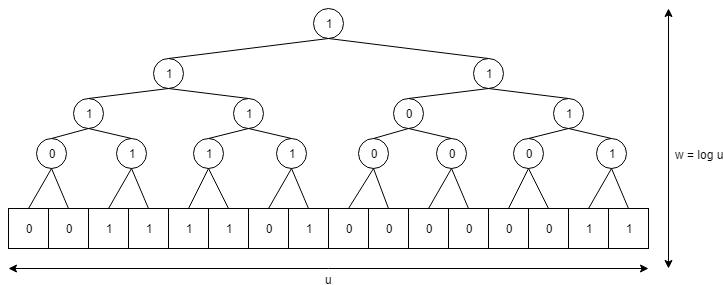
\includegraphics[width=0.9\textwidth]{stratified-tree.png}
\end{figure}

\subsubsection{van Emde Boas trees}

The van Emde Boas\index{van Emde Boas} trees is a data structure which can be seen as a tree with high degree and defined recursively. It is composed of two elements:
\begin{itemize}
    \item Clusters: Each cluster holds $\sqrt{u}$ subclusters and this recursively until it contains all the elements of the universe.
    \item Summary: Each cluster is summarized by one element which will help to guide the path to the predecessor or successor element. It is also recursively defined since the summary summarizes the information of its subtree.
\end{itemize}

The whole point is that we can access these helper structures in constant time due to the definition of our tree where the index of the cluster can be easily computed at each step. Hence, the cluster and its relative offset is defined as $(\frac{x}{\sqrt{u}}, x \text{ mod } \sqrt{u})$ which in the case of binary numbers leads to: $(\frac{x}{2^{\frac{w}{2}}}, x \text{ mod } 2^{\frac{w}{2}})$ which are roughly a shift and a mask operations.

\begin{figure}[!h]
   \caption{vEB idea}
   \label{vEB}
   \centering
   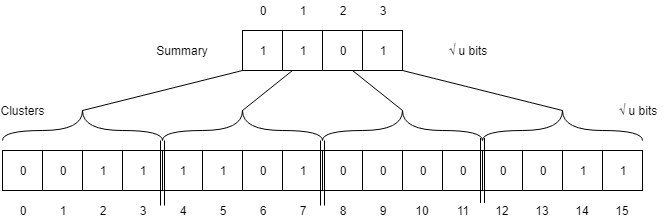
\includegraphics[width=0.9\textwidth]{vEB.png}
\end{figure}

K. Melhorn and S. Näher~\cite{mehlhorn1990bounded} proved that we can achieve $O(N)$ memory if we use hash tables\index{Hash table} which map prefix of the integers to ordered linked-list nodes while preserving complexity with high probability. An idea similar to Y-fast tries can also be applied for this purpose.

\subsection{X/Y-fast tries}

The problem with the \textit{van Emde Boas}\index{van Emde Boas} trees is that they consume a huge amount of memory. D. E. Willard~\cite{willard1983log}, in 1982, proposed two solutions to this problem based on the stratified tree idea. The first part of its answer is called the \textit{X-fast} trie, the idea is rather simple, only store the present elements, whose bit are set to one. We save the path to the node (with left as 0 and right as 1, for example) in a dynamic hash table, called level-search structure, and we associate it with the minimal/maximal value of the subtree. So instead of directly jumping to the subtree, we ensure the presence thanks to the hash table. This technique consumes $O(N \log u)$ memory to store each elements and their binary representation (note that we can spare some space since a common prefix/suffix is shared). Also, we may need to update a whole path, up to $O(\log u)$ values but we can achieve predecessor/succesor queries in $O(\log \log u)$ with high probability and search for one specific elements in $O(1)$. We can also maintain a linked list of the entire set of occupied leaves, this allows that given node x, we can find the successor and the predecessor in $O(1)$.

Second, we gain a lot of space, but we lose the $O(\log \log u)$ on insert and delete. Hopefully, the \textit{Y-fast} trie are there. They consist of two layers, the summit of the trie is made of a \textit{X-fast} trie such that it holds $\Theta(\frac{N}{\log u})$ elements and the leaves are other canonical binary seach trees of $O(\log u)$ elements where one representant is placed in the upper trie. This thus achieves the $O(N)$ in space and the operations are bound by $O(\log \log u)$ in the bottom trees since the update time is dominated by the leaf structures. Complexity is exchanged throughout the structure by amortizing it into the terminal elements.

Finally, let's conclude by saying that this data structure even though has nice properties, we may prefer to implement a \textit{X-fast} trie which are simpler to code and more efficient in practice. We need also to emphasize on the fact that the performances of this tree depends heavily on the hash table performances and the time to insert one element can thus vary by a huge factor. Notice that the complexity is not optimal, it is expected to be $O(\frac{\log \log u}{\log \log \log u})$ for $N^{O(1)}$ space~\cite{patracscu2007randomization}. Other data structures based on similar concepts have been developed to address the problem of the predecessor or the dynamic least common ancestor~\cite{bose2013fast,belazzougui2009monotone}. You may also be interested in the little brother of this data structure, defined in the $AC^{0}$ computation model (constant depth circuit which behaves as word-RAM like without multiplication), and called \textit{fusion tree}~\cite{fredman1990blasting}.


\section{X-fast trie}

Following the various observations we made in the two previous chapters, we finally embarked on different implementation for the X-fast tries\index{X-fast trie}. All share a common base, the trie is seen, on the one hand, as a set of intermediate levels that allow to navigate in the trie and determine which is the predecessor or successor of an element depending of its prefix and, on the other hand, a last level actually containing the key-value pairs.

All of these rely on the use of a hash table\index{Hash table}, based on the open-addressing\index{Open addressing} principle and with the linear probing\index{Probing} strategy for the implementation, we will come back to these notions in the forthcoming chapter$ ^{[\ref{Hash table}]}$. We have thought about different ways to build and operate on these and we have identified three main implementation families:

\subsection{Binary search\index{Binary strategy}}

In order to find out from which height the new nodes should be inserted, a simple dichotomous search is performed on the levels. This introduces a natural complexity in $O(\log \log u)$ on the search for the predecessor/successor. However, the entire warp is used for this task since this treatment is inherently sequential. Once the lowest node has been found, all that remains is to complete the trie and update the parents as long as necessary.

We have tried to show the different steps performed by these different implementations with their respective time indication. The search for nodes is symbolized by the {\color{black}black} color, the insertion of new nodes is tinted {\color{green}green} and the update of the parents is {\color{red}red}. The arrows represent which levels are actually accessed. And the number defines the order of execution, a same number indicating parallelism of the task.

For this, we decided that the whole warp should contribute to the task, the idea was that when we do our research for a particular new location or object in the hash table\index{Hash table}, the different threads will access the following probes at once. This allows all threads to perform the same task and therefore there is no divergence and thus variance is minimized. This is done at the cost of more total data access. We update the parents as long as the minimum/maximum of their subtrees is not affected by our new element.

\begin{figure}[!ht]
\centering
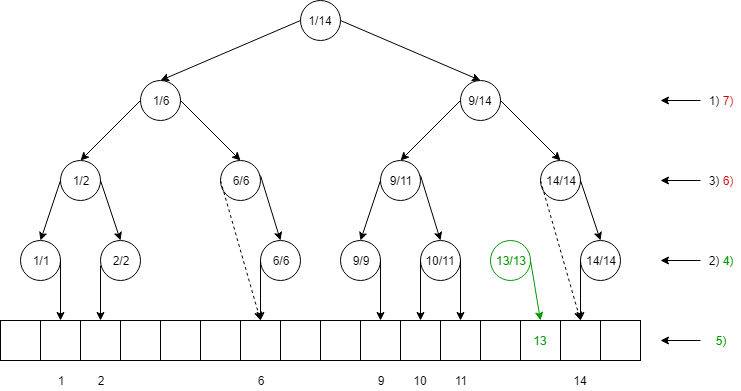
\includegraphics[width=\linewidth]{Chapters/XFastTries/Implementation/BinaryStrategy.png} 
\caption{Binary strategy}
\end{figure}

\subsection{Warp search\index{Warp strategy}}

The previous technique is unnecessarily inefficient, all queries that resulted in the absence of a prefix cannot be used effectively and the gain provided by a successful query is marginal. This is why, and following the observations on memory accesses, we opted for each thread to make an independent request on a particular level. All levels are therefore read at once and thanks to the election mechanisms in warps, the lowest level is determined at once.

The voting functions\index{Warp voting} in warps allow all threads in a warp to perform a broadcast operation followed by a reduction in a single step and at very high speed. These take as input an integer that will serve as predicate, all threads will then compare their own value with that provided, the comparison results are combined and sent to each participant. It is then enough to recover the position of the bits set to one to know for which threads the predicate was true.

Now that we have found the lowest node, the first part will update the parents simultaneously with each time only one thread associated to a level and the other part will insert the new ones in the same way. However, care must be taken to resize these hash tables\index{Hash table}. Indeed, either we can resize the hash table\index{Hash table} when we deem it necessary or we can work with ``amortized'' operations, each time we insert an element, we take the opportunity to transfer elements from the old table to the new one. In our case, we opted for the first approach which is simpler to implement and a preliminary step is thus taken to determine whether there is still enough space. We will come back to this aspect later.

\begin{figure}[!ht]
\centering
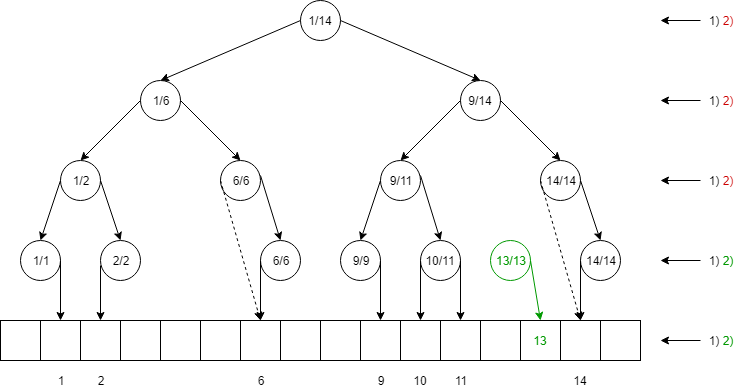
\includegraphics[width=\linewidth]{Chapters/XFastTries/Implementation/WarpStrategy.png} 
\caption{Warp strategy\index{Warp strategy}}
\end{figure}

\subsection{Group search\index{Group strategy}}

After implementing the warp search\index{Warp strategy} idea, it seemed quite natural to look for a subset of the trie instead of one and only one element. Those will be stored as a simple array in their associated parent, to mimick a structure close to the one we find out in van Emde Boas layouts which grant search in less than $O(4 \log_{B} N)$ memory transfers~\cite{bender2005cache}. This would store fewer elements in total and therefore consume less memory, but it is not the only advantage. This also reduces the number of line caches\index{Block} needed to fill all queries and also decreases the likelihood of falling into a worst case scenario with a degenerate item search case in a hash table\index{Hash table}. In addition, warp access will respond to more levels and therefore require a lower number of total accesses in the end. If we use 64-bit keys, the warp strategy\index{Warp strategy} will require two accesses whereas the group strategy, even with a group size of 1, only one will be enough to fullfill the request.

Here, we define group size as the number of levels and therefore children that are grouped into a single entity that will serve as a value. One bit and all its prefix will serve as the key. Care must be taken to update these elements in accordance with their memory layout. It is also necessary to ensure that both operations of update and insertion are done within the same group when the lowest node falls inside a group. Warp search\index{Warp strategy} can be seen as a special case of group search when the group size is equal to 0.

\begin{figure}[!ht]
\centering
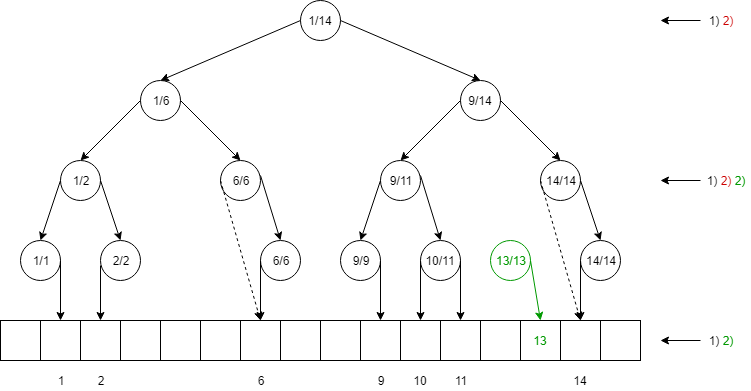
\includegraphics[width=\linewidth]{Chapters/XFastTries/Implementation/GroupStrategy.png} 
\caption{Group strategy - group of size 1}
\end{figure}

\subsection{Experiment}

We set up an experimental protocol in order to compare the various possible strategies to implement an X-fast trie\index{X-fast trie}. This consists in pre-allocating a large memory area, attaching to it a memory allocator (so called ``linear'') that works by assigning the next memory area each time, so the allocations are constant time and disallocation operations are equivalent to no operations, and from which we will pick for our problem. We then build our tries by preallocating enough memory to contain all our insertions, this is done in order to provide a more independent result on the hash tables used. We will see that there is some flexibility on hash table\index{Hash table} and that more complex implementations can remain competitive and interesting in practice.

Once our tries are well built, variables correctly initialized and so on, we insert a large amount of elements and we measure the time taken on an average of 10 runs with 10 iterations. Each run receives its associated and random seed which will be used to feed a pseudo random generator (hash function) based on the current index of the insertion and the associated seed which will generate the distribution of keys for the elements to insert. We do similar work to test search operations. We pre-construct our tries and pre-fill them with enough elements, and we measure the time taken to answer all our successful requests, both by making requests by warp (the 32 threads are used to answer the same key) and by thread (each thread looks for the value associated with a different key). Finally, the same experiment is done but for the predecessor and successor queries; the look-up keys are created as a combination of the random numbers and the original seed, we may expect to have low exact match on the keys. Remark that only one warp is active in those experiments, no concurrency\index{Concurrent} is made.

\subsection{B+ Tree\index{B-tree}}\label{BTREE}

In order to see the performance of our data structure, it was interesting to implement another one that shares the same operations and similar properties. We opted for B+ trees\index{B-tree}~\cite{comer1979ubiquitous} which is the trie version of the classical B-trees\index{B-tree}, introduced by R. Bayer and E. M. McCreight in 1971. Indeed, it is a very classical associative data structure which has the operations which interest us the insertions/deletions/searches and predecessor/successor queries, which has been widely studied for its good properties~\cite{bender2005cache} and which was ported successfully on GPU\index{Graphics cards}~\cite{fix2011accelerating}. B-trees\index{B-tree} can be seen as generalizations of binary search trees where instead of having only two children, we have B children; it is also self-balancing. This naturally gives complexities in $O(\log_{B} N)$ for many dynamic operations.

We decided to present B+-trees instead of B-trees\index{B-tree} because they seem, for us, conceptually simpler and the algorithms are essentially the same. They have the advantage of being cleaner and not mixing two different notions. The letter $m$ will design the number of children in one node in this section.

A B+-tree\index{B-tree} is a rooted tree having two kind of nodes:
\begin{itemize}
    \item Internal node: are made of $m - 1$ keys ordered with $m$ associated pointers linking either to another internal node or a leaf node. Those keys are meant to separate the ranges of keys stored in each subtree.
    \item Leaf node: are made of $m$ keys ordered with $m$ associated values.\\
\end{itemize}

The B+-trees\index{B-tree} obey these following properties~\cite{comer1979ubiquitous}:
\begin{itemize}
    \item Every node has at most $m$ children.
    \item Every non-leaf node (except root) has at least $\lceil \frac{m}{2} \rceil$ children.
    \item The root has at least two children if it is not a leaf node.
    \item A non-leaf node with $k$ children contains $k-1$ keys.
    \item All leaves appear at the same level.\\
\end{itemize}

Searching in a B+ tree\index{B-tree} is similar to searching in a binary search tree, except instead of making a binary decision at each node, we make a multiway branching decision based on the number of children in that node and our look-up key. A simple binary search can be done on the keys of one node.

Inserting a new element into a B+-tree\index{B-tree} is more complicated than inserting a key into a binary search tree. We start with a similar step where we look for the leaf position where to insert our new element and we insert the new key into an existing leaf node. However, we cannot insert an element when the leaf is full. For that, a special operation called soberly ``split'' is carried out, it consists in dividing the number of children of the leaf in two new leaves. The middle key will be moved to the parent internal node to identify the split point between the two new trees. But if the parent is also full, we have to divide it before we can insert the new key, and so we might end up dividing over the entire height of the tree.

Deletion is a bit trickier, there are two main strategies, either we locate and delete the item, then restructure the tree to retain its invariants or while going down the tree, we restructure the nodes such that the invariants are kept and when we encounter the final element, we can simply remove it without breaking any invariants. We must also pay attention to two particular cases, if the key is used as a separation element between two nodes or if this is the minimum/maximum of a leaf-node. In these two cases, it will also be necessary to update the parent's keys.

\begin{figure}[!ht]
\centering
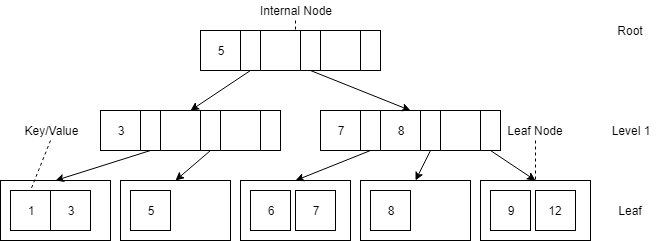
\includegraphics[width=\linewidth]{Chapters/XFastTries/Implementation/BTree.png} 
\caption{B+Tree representation with $m = 3$}
\end{figure}

The essential difference between B-trees and B+-trees\index{B-tree} is this mixture between values and pointers in intermediate nodes, otherwise their structure is really similar. We opted for the B+ trees\index{B-tree} variant instead of the simple B trees\index{B-tree} because they allow to group keys and pointers and thus to guarantee a better distribution of data within the levels but keys are then copied at several places. The distinction between values and pointers is also more clear and avoid some cumbersome detail of implementation. We opted to set the number of children of one node to $m = 32$, because it allows to get the child or the position to insert at once thanks to the voting\index{Warp voting} system in the warps. Each thread can possibly compare with its associated key in the node at once.

\subsection{Results}

We will start by presenting the results obtained for the insertions, we will follow by the two different search operations and we will end with the predecessor/successor queries. Each time, we will discuss the results, notice the potential improvements or elaborate on points which seem more relevant to our case. The graphs should be interpreted as the mean time taken to perform the number of operations (described by the head of the row) with the standard deviation between parentheses and the strategy per column, the intermediate rows represent the ratio between the time taken by the B-tree and the X-fast trie\index{X-fast trie} strategy (the lower the number is, the better the strategy is). All these times are expressed in microseconds (µs):

\subsubsection{Insertions}

We performed the experiment twice, once with 32-bit keys and once with 64-bit keys. After running our experiments and extracting the data here is what we got:

\begin{table}[!h]
\centering
\caption{Time to insert K elements with all these strategies with 32-bit keys (in µs)\\
mean time (standard deviation) - intermediate lines represent slowdown factor}
\label{32bitsInsertions}
\resizebox{\columnwidth}{!}{%
\begin{tabular}{cccccccc}
Insertion & B-tree        & Binary       & Group1       & Group2       & Group3       & Group4       & Warp         \\
1024      & 3064 (30)    & 6053 (21)    & 1691 (13)    & 1695 (16)    & 1736 (11)    & 1830 (16)    & 1593 (13)    \\
          &              & 1.98         & 0.55         & 0.55         & 0.57         & 0.6          & 0.52         \\
2048      & 6024 (17)    & 11823 (45)   & 3438 (30)    & 3434 (22)    & 3554 (20)    & 3740 (15)    & 3242 (23)    \\
          &              & 1.96         & 0.57         & 0.57         & 0.59         & 0.62         & 0.54         \\
4096      & 11986 (15)   & 22974 (60)   & 6884 (18)    & 6969 (24)    & 7148 (26)    & 7529 (25)    & 6517 (13)    \\
          &              & 1.92         & 0.57         & 0.58         & 0.6          & 0.63         & 0.54         \\
8192      & 23916 (30)   & 44515 (127)  & 13682 (41)   & 13856 (34)   & 14257 (23)   & 15043 (35)   & 12972 (28)   \\
          &              & 1.86         & 0.57         & 0.58         & 0.6          & 0.63         & 0.54         \\
16394     & 65411 (181)  & 86178 (223)  & 27219 (40)   & 27726 (40)   & 28571 (52)   & 30107 (55)   & 26091 (49)   \\
          &              & 1.32         & 0.42         & 0.42         & 0.44         & 0.46         & 0.4          \\
32768     & 133339 (254) & 167413 (444) & 55193 (81)   & 56032 (85)   & 57656 (84)   & 60546 (88)   & 52708 (72)   \\
          &              & 1.26         & 0.41         & 0.42         & 0.43         & 0.45         & 0.4          \\
65536     & 268613 (581) & 320465 (932) & 114746 (172) & 116848 (158) & 119413 (169) & 124226 (169) & 107993 (173) \\
          &              & 1.19         & 0.43         & 0.44         & 0.44         & 0.46         & 0.4       
\end{tabular}
}
\end{table}

\begin{table}[!h]
\centering
\caption{Time to insert K elements with all these strategies with 64-bit keys (in µs)}
\label{64bitsInsertions}
\resizebox{\columnwidth}{!}{%
\begin{tabular}{cccccccc}
Insertion & B-tree       & Binary       & Group1       & Group2       & Group3       & Group4       & Warp         \\
1024      & 3079 (34)    & 6743 (26)    & 1893 (13)    & 1900 (11)    & 1966 (12)    & 2087 (20)    & 1837 (17)    \\
          &              & 2.19         & 0.61         & 0.62         & 0.64         & 0.68         & 0.6          \\
2048      & 6131 (16)    & 12947 (40)   & 3749 (31)    & 3818 (29)    & 3949 (26)    & 4110 (29)    & 3647 (32)    \\
          &              & 2.11         & 0.61         & 0.62         & 0.64         & 0.67         & 0.59         \\
4096      & 12181 (24)   & 24979 (61)   & 7413 (30)    & 7555 (20)    & 7840 (22)    & 8157 (19)    & 7197 (28)    \\
          &              & 2.05         & 0.61         & 0.62         & 0.64         & 0.67         & 0.59         \\
8192      & 24330 (32)   & 48336 (114)  & 14914 (31)   & 14987 (26)   & 15552 (29)   & 16384 (28)   & 14360 (22)   \\
          &              & 1.99         & 0.61         & 0.62         & 0.64         & 0.67         & 0.59         \\
16394     & 67532 (179)  & 93456 (209)  & 29936 (44)   & 30062 (43)   & 31192 (38)   & 32945 (68)   & 28925 (30)   \\
          &              & 1.38         & 0.44         & 0.45         & 0.46         & 0.49         & 0.43         \\
32768     & 137071 (297) & 181747 (442) & 60658 (78)   & 61541 (106)  & 63654 (89)   & 66154 (95)   & 58915 (72)   \\
          &              & 1.33         & 0.44         & 0.45         & 0.46         & 0.48         & 0.43         \\
65536     & 279735 (544) & 349635 (824) & 126038 (165) & 126811 (179) & 130452 (166) & 135358 (198) & 121929 (184) \\
          &              & 1.25         & 0.45         & 0.45         & 0.47         & 0.48         & 0.44        
\end{tabular}
}
\end{table}

We can make different observations in view of the results obtained:
\begin{itemize}
    \item The strategy of doing a dichotomous search (Binary\index{Binary strategy}) on levels is always slower. Indeed, it is very inefficient in the way the elements are accessed. The gain brought by adjacent accesses does not compensate for their very large number, random accesses are more interesting in this case.
    \item The time to insert elements is almost linear in all cases, there is a big exception for B-trees\index{B-tree} when you go from 8192 ($2^{13}$) elements to 16834 ($2^{14}$). Indeed, this corresponds to the transition between three and four levels in the tree with all the rebalancing that this induces due to the fact that with used B-trees\index{B-tree} with $m = 32$ (to correspond to the size of a warp).
    \item The time to perform 64-bit insertions isn't much higher, about 3 percent for B-trees and 5 percent for the others (GroupK\index{Group strategy} and Binary\index{Binary strategy}), except for warp insertions\index{Warp strategy} which go up to 8 percent. The time is expected to be roughly constant for B-trees\index{B-tree} since their operation is independent of the size of the key. Group strategies\index{Group strategy} benefit from the fact that a single warp allows access to all 63 levels at once since we ask for at least two levels at once, while the warp strategy\index{Warp strategy} requires two accesses.
    \item More importantly, GroupK\index{Group strategy} and Warp strategies\index{Warp strategy} show a real gain over B-trees\index{B-tree} when a large number of insertion requests are made. This supports the observations made on memory access$^{[\ref{Accesses}]}$ and the idea that B-tree\index{B-tree} requires $O(\log_{B}N)$ sequential\index{Sequential} accesses while X-fast tries\index{X-fast trie} only require $O(\lceil \frac{\log U}{32} \rceil)$ accesses but random. The standard deviation also tends to be lower than for B-trees\index{B-tree} since potential rebalancing is avoided.
    \item Group strategy\index{Group strategy} with group size of $1$ or $2$ and warp strategy\index{Warp strategy} presents the best performances for this operation and presents a large improvement compared to the B-tree\index{B-tree} reference structure.
\end{itemize}

\subsubsection{Search}

And this is what we collected for the search operation for those both experiments, those per warp where all the threads in a warp are used to find an element and those per thread where each thread searches for its own element:

\begin{table}[!htb]
    \caption{Time to get K elements with 64-bit keys (in µs)}
    \begin{minipage}{.5\linewidth}
      \label{getbywarp}
      \caption{By warp}
      \centering
\begin{tabular}{ccc}
Search by warp & B-tree   & Warp       \\
1024    & 1960 (38)    & 781 (22)   \\
        &              & 0.4        \\
2048    & 3812 (31)    & 1579 (14)  \\
        &              & 0.41       \\
4096    & 7480 (15)    & 2997 (18)  \\
        &              & 0.4        \\
8192    & 14866 (22)   & 5904 (17)  \\
        &              & 0.4        \\
16394   & 46063 (111)  & 11663 (11) \\
        &              & 0.25       \\
32768   & 91482 (213)  & 23237 (22) \\
        &              & 0.25       \\
65536   & 186031 (383) & 46180 (23) \\
        &              & 0.25      
\end{tabular}
    \end{minipage}%
    \begin{minipage}{.5\linewidth}
      \centering
        \caption{By thread}
\begin{tabular}{ccc}
Search by thread & B-tree      & Warp      \\
1024          & 256 (31)    & 101 (16)  \\
              &             & 0.39      \\
2048          & 462 (48)    & 142 (19)  \\
              &             & 0.31      \\
4096          & 879 (92)    & 180 (8)   \\
              &             & 0.2       \\
8192          & 1651 (153)  & 329 (5)   \\
              &             & 0.2       \\
16394         & 3354 (197)  & 690 (7)   \\
              &             & 0.21      \\
32768         & 6769 (245)  & 1606 (30) \\
              &             & 0.24      \\
65536         & 14642 (270) & 4278 (35) \\
              &             & 0.29     
\end{tabular}
    \end{minipage} 
\end{table}

Let's start by saying that we mentioned the results only for one of the strategies implemented for X-fast tries\index{X-fast trie} since all have the same underlying hash table\index{Hash table} for the elements at the bottom. The differences in results were therefore marginal (less than 0.1\%) and not significant according to a paired t-test and common sense.
Once again, we obtained very interesting results:

\begin{itemize}
    \item ``search by warp'' for X-fast tries\index{X-fast trie} is much faster than for B-trees\index{B-tree}, the standard deviation is also much smaller since we have to do $O(\log_{B}N)$ access for B-trees\index{B-tree} and $O(1)$ for X-fast tries\index{X-fast trie} with high probability by the intrinsic properties of these structures.
    \item ``search by threads'' are also magnitude faster for a lower standard deviation. This is explained by the number of accesses required for B-trees\index{B-tree} which are $O(\log_{B}N * \log_{2}B)$ since we have to perform a dichotomous search on the keys while they remain in $O(1)$ for X-fast tries\index{X-fast trie}.
    \item The speed-up ratio to access data per thread compared to warp is only about 12 for B-trees\index{B-tree} and over 12 for X-fast tries\index{X-fast trie}. This is consistent with the observation that random access is still more attractive than performing the equivalent number of sequential\index{Sequential} accesses.
    \item An increasing standard deviation can be expected for B-trees\index{B-tree} as a function of the number of queries made, given the number of possible branches in thread accesses greater than for hash table\index{Hash table} accesses which remain consistent and proportional to the load factor.
    \item The time required to access items per thread is not directly proportional to the number of queries made due to the characteristics of our hash table\index{Hash table}, the greater the load factor, the longer can be expected to retrieve one element.\\
\end{itemize}

\subsubsection{Predecessor/Successor}

Next, we need to analyze the results related to the requests of predecessors and successors:

\begin{table}[!htb]
\centering
\caption{Predecessor queries on 64-bit keys}
\resizebox{\columnwidth}{!}{%
\begin{tabular}{cccccccc}
Predecessor & BTree        & Binary       & Group1       & Group2       & Group3       & Group4       & Warp         \\
1024        & 2634 (33)    & 8235 (34)    & 2851 (24)    & 4729 (29)    & 4842 (38)    & 4984 (25)    & 4249 (37)    \\
            &              & 3.13         & 1.08         & 1.8          & 1.84         & 1.89         & 1.61         \\
2048        & 5145 (18)    & 16342 (41)   & 5629 (14)    & 9507 (35)    & 9775 (42)    & 10016 (41)   & 8520 (33)    \\
            &              & 3.18         & 1.09         & 1.85         & 1.9          & 1.95         & 1.66         \\
4096        & 10124 (20)   & 32645 (50)   & 11387 (19)   & 19227 (47)   & 19659 (59)   & 19946 (63)   & 17208 (48)   \\
            &              & 3.22         & 1.12         & 1.9          & 1.94         & 1.97         & 1.7          \\
8192        & 20157 (19)   & 65276 (39)   & 23387 (28)   & 38884 (44)   & 39746 (42)   & 40349 (49)   & 35276 (39)   \\
            &              & 3.24         & 1.16         & 1.93         & 1.97         & 2.0          & 1.75         \\
16394       & 53144 (121)  & 130700 (66)  & 49046 (36)   & 79847 (66)   & 82120 (77)   & 83651 (72)   & 73536 (78)   \\
            &              & 2.46         & 0.92         & 1.5          & 1.55         & 1.57         & 1.38         \\
32768       & 105540 (212) & 262535 (97)  & 108955 (78)  & 171596 (148) & 174387 (101) & 178055 (127) & 159783 (134) \\
            &              & 2.49         & 1.03         & 1.63         & 1.65         & 1.69         & 1.51         \\
65536       & 214314 (571) & 525281 (164) & 305071 (853) & 431696 (610) & 426686 (496) & 428355 (534) & 431530 (745) \\
            &              & 2.45         & 1.42         & 2.01         & 1.99         & 2.0          & 2.01        
\end{tabular}
}
\end{table}

\begin{table}[!htb]
\centering
\caption{Successor queries on 64-bit keys}
\resizebox{\columnwidth}{!}{%
\begin{tabular}{cccccccc}
Successor & BTree        & Binary       & Group1       & Group2       & Group3       & Group4       & Warp         \\
1024      & 2381 (25)    & 8137 (31)    & 2850 (35)    & 4655 (30)    & 4750 (39)    & 4929 (41)    & 4156 (26)    \\
          &              & 3.42         & 1.2          & 1.96         & 2.0          & 2.07         & 1.75         \\
2048      & 4680 (20)    & 16135 (35)   & 5623 (31)    & 9388 (52)    & 9577 (24)    & 9885 (41)    & 8310 (54)    \\
          &              & 3.45         & 1.2          & 2.01         & 2.05         & 2.11         & 1.78         \\
4096      & 9174 (19)    & 32270 (47)   & 11355 (33)   & 18982 (48)   & 19221 (60)   & 19642 (74)   & 16845 (58)   \\
          &              & 3.52         & 1.24         & 2.07         & 2.1          & 2.14         & 1.84         \\
8192      & 18305 (18)   & 64561 (51)   & 23319 (31)   & 38360 (38)   & 38878 (76)   & 39730 (99)   & 34595 (52)   \\
          &              & 3.53         & 1.27         & 2.1          & 2.12         & 2.17         & 1.89         \\
16394     & 49485 (122)  & 129250 (77)  & 48912 (30)   & 78756 (103)  & 80659 (110)  & 82431 (101)  & 72079 (74)   \\
          &              & 2.61         & 0.99         & 1.59         & 1.63         & 1.67         & 1.46         \\
32768     & 98362 (264)  & 260552 (249) & 108610 (97)  & 169961 (173) & 171513 (202) & 176271 (142) & 156794 (162) \\
          &              & 2.65         & 1.1          & 1.73         & 1.74         & 1.79         & 1.59         \\
65536     & 200266 (392) & 521108 (173) & 304131 (872) & 428136 (702) & 420038 (699) & 424094 (721) & 426341 (642) \\
          &              & 2.6          & 1.52         & 2.14         & 2.1          & 2.12         & 2.13        
\end{tabular}
}
\end{table}

The results are somewhat surprising. We can observe different elements:
\begin{itemize}
    \item All times are directly proportional to the number of elements queried, which is expected.
    \item The time required to perform predecessor/successor queries in B-trees\index{B-tree} is roughly equivalent to the search operations. This is quite natural by the nature of tree search. There is also a slight difference between the two types of queries since the same dichotomous search was performed while in one case one looks for a lower bound and in the other an upper bound on the keys. The treatment is therefore a bit dissimilar between the two cases, but can easily become the same. While the treatment is the same in both the case for the X-fast tries\index{X-fast trie}.
    \item X-fast tries\index{X-fast trie} are significantly slower than B-trees\index{B-tree} by a factor 2 ! This result is somewhat surprising when you consider that, for the X-fast tries, the time taken to insert elements is roughly the same. Accessing the different levels seems to be quite logically the limiting factor.
    \item We were expecting a certain slowness related to this global look-up followed by the two potential hash table\index{Hash table} searches (when we search for the predecessor and there is no left subtree for example) that are being done but not to this point. Perhaps an element escaped our re-reading of the code and a pessimisation slipped in. The other explanation being that it is the rebalancing in the tree which strongly degraded the performances of B-tree\index{B-tree}. Operation that simply does not exist for queries.
    \item One should not be worried due the presence of an exacerbated difference in performance between size 1 and 2 groups\index{Group strategy}; but this is simply due to the fact that we can not fit all the elements in a single cache\index{Block} line with group of size more than 1. The results are roughly equivalent with queries on 32-bit keys and only the strategy of grouping by size of 1 seems really effective.\\
\end{itemize}

\subsubsection{Memory consumption}

Finally, all that remains is to analyze the memory consumption of such data structure. We have tried to make a approximate calculation on the memory consumption of these different structures. Let us begin by describing the assumptions we have made:
\begin{itemize}
    \item The size of the keys for both B+-trees\index{B-tree} and X-fast tries\index{X-fast trie} is the same, and this applies to the internal nodes as well as the leaves or the intermediate and bottom levels. If we have an X-fast tries\index{X-fast trie} of 32 levels, the keys are 32 bits, or 4 bytes.
    \item We set the size of the pointers contained in the intermediate nodes to 8 bytes.
    \item The hash tables\index{Hash table} used are twice as large as the number of elements they can accommodate. And the resizing takes place when the load factor reaches 50\% (in order to simplify the calculations and to have only powers of 2).
    \item The size of the values was fixed at 4 bytes but this data only intervenes for the leaves or the bottom level.
    \item The B-tree\index{B-tree} contains $m = 32$ children per node.\\
\end{itemize}

We will start by explaining the calculation performed for B+-trees\index{B-tree}:\\
If we have N randomly distributed elements in the leaves, then we have $\lceil \frac{N}{B} \rceil$ leaf nodes. Since internal nodes have potentially up to B children, the tree size is simply $\log_{B} N$ and there are thus $\lceil \frac{N}{B} \rceil * \log_{B} N$ elements in total. The number of intermediate nodes is therefore this quantity minus the number of leaves. So the total amount of memory is proportional to:
$$ \lceil \frac{N}{B} \rceil * B * \text{(key size + value size)} +( \lceil \frac{N}{B} \rceil * \log_{B} N - \lceil \frac{N}{B} \rceil) * B * \text{(key size + pointer size)} $$

And now for the X-fast tries\index{X-fast trie}:\\
Under the previous assumptions, we know that the size of a hash table\index{Hash table} containing $N$ element corresponds to the next power of $2$. Second, the intermediate level $i$ contains at most $2^{i}$ elements since only the first $i$ bits are read and, in group strategies\index{Group strategy}, those nodes have at most $2^{k}$ (where $k$ is the group size) children layout in van Emde Boas fashion. If we define the height of the tree as $w$; the computation resumes to:

\lstinputlisting[language=Python]{Chapters/XFastTries/Implementation/memory_xfasttries.py}

Now if we ask to draw these two functions with fixed parameters in comparison with the actually required memory, here is what we get:

\begin{figure}[!ht]
\centering
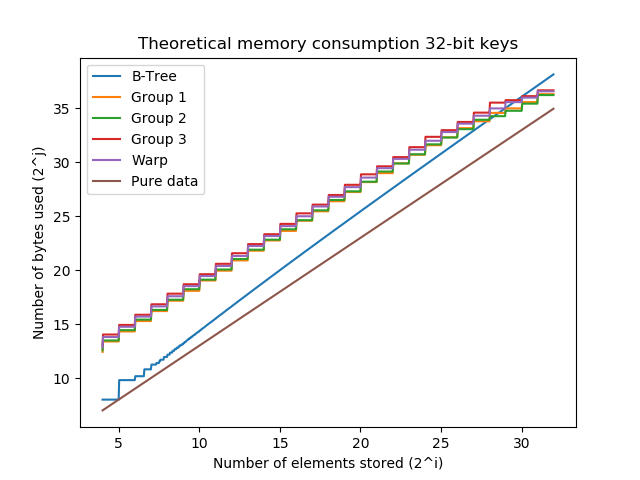
\includegraphics[width=0.925\linewidth]{Chapters/XFastTries/Implementation/MemoryConsumption32.png} 
\caption{Memory consumption in bytes with $m = 32$ and 32-bit keys}
\end{figure}

We observe that X-fast tries\index{X-fast trie} consume proportionally much more memory than B+-trees\index{B-tree} and that it takes a lot of elements before they are competitive. At first glance, it's not obvious that this trend exists but let's not forget that B+-trees\index{B-tree} have a $O(\log_{B}N)$ factor compared to linear. Second, hash tables\index{Hash table} tend to have a consumption directly proportional to the number of items $\Theta(n)$. However, the problem is that we initially have a very large number of hash tables\index{Hash table} that require resizing but this proportion is decreasing since those located near the root have reached their final size and will not be able to grow any further. Here, group size of $1$ and $2$ manage to reduce overall memory consumption compared to other strategies for X-fast tries\index{X-fast trie}.

\subsubsection{Conclusion}

The data structure seems to offer some really interesting features. The insertion and search requests are much faster than the reference structure used here which proposes some common properties. However, time is wasted on requests from predecessors/successors but within acceptable time frames. It is thus really adapted if the requests for insertions or obtentions are more common than those of predecessor/successor. Note that it also seems difficult to propose insert operations or predecessor/successor requests if we only have one available thread for the X-fast tries\index{X-fast trie} while it remains feasible with B-tree\index{B-tree}.

But before we get any more excited, we must first realize that the results obtained for X-fast tries\index{X-fast trie} are terribly dependent on the hash table\index{Hash table} used. Here, enough space has been allocated in advance to avoid a possible resizing of the table that could drastically reduce performance. In our experimental case, we used an open-addressing\index{Open addressing} hash table\index{Hash table} with linear probing\index{Probing} and a 75 percent load factor. We also notice that the time to obtain elements is not linear in the number of queries, this corresponds to the fact that the number of probes required to find an element can be expressed on average as a function of the load factor. On the other hand, the B-tree\index{B-tree} node allocation policy is also very simplified and can be summarized as a single operation (an addition on a pointer).

The results were also obtained in a very particular case where only one warp was being executed; which is very far from the case of traditional use of a graphics card. This is therefore more of a proof of concept since the structure was not built to be concurrent\index{Concurrent}. But let's not be so defeatist, the concurrent\index{Concurrent} possibilities of X-fast tries\index{X-fast trie} are higher than for B-trees\index{B-tree} given the problems related to rebalancing and root management. Much literature exists on effective ways to make hash tables\index{Hash table} concurrent\index{Concurrent}~\cite{maier2016concurrent} but less on the B-trees\index{B-tree} seen their inherent difficulty~\cite{braginsky2012lock}.


\appendix
\chapter{Implementation details}

This chapter will be devoted to themes that are related to the purpose of this work but that do not directly support it. This presents more technical aspects, which certainly have an impact on our conclusions, but which are a bit off. They remain important to notify in order to reproduce the experiences but less assiduous readers can stop reading here. We will start by detailing the hardware used in the experiments and then move on to the specific software used. Everything has been developed in C++-14, since this is the maximum version supported by CUDA 9.1.


\section{Hardware}

All experiments were performed on the same computer. This nearly last generation material made it possible to benefit from the lastest innovations, in particular those related to the principle of election in the warps. Here are described the components:

\begin{table}[!ht]
\centering
\caption{Components}
\begin{tabular}{lll}
Hardware    &                                 &  \\
GPU         & GTX 1050 ti                     &  \\
CPU         & AMD Ryzen 5 1600                &  \\
Memory      & G.SKILL Ripjaws V Series 2x8 GB &  \\
SSD         & Samsung SSD 850 EVO 250GB       &  \\
Motherboard & ASRock AB350M Pro4              & 
\end{tabular}
\end{table}

In practice, this graphics card offers compute capabilities 6.1 with 6 multiprocessors consisting of:
128 CUDA cores for arithmetic operations, 32 special function units for single-precision floating-point transcendental functions, and 4 warp schedulers. Each multiprocessor has a shared memory of 96KB (divided into registers and shared data).
There is also a L1 cache for each multiprocessor and a L2 cache shared by all multiprocessors that is used to cache accesses to local or global memory, including temporary register spills.\\
All this can offer, in theory, up to 2 TFLOPS with a global memory bandwidth of 112GB/s. In practice, the performances are often lower than the theoretical ones announced by the manufacturer.


\section{Software}

The version of these softwares can also have an impact on the performance obtained:

\begin{table}[!ht]
\centering
\caption{Software versions}
\label{my-label}
\begin{tabular}{lll}
Software   &                                                             &  \\
OS         & Microsoft Windows 10 Professional 64 bit (build 10.0.16299) &  \\
GPU driver & GeForce driver 391.35                                       &  \\
CUDA       & CUDA Toolkit v9.1.85                                        &  \\
Compiler   & Visual studio 2017 version 15.4.5 (C++)                     & 
\end{tabular}
\end{table}

We also tested our software under Ubuntu 17.10 but following various problems related to drivers not adapted, most of the development was done under Windows 10.


\section{Libraries}

To develop our software and experiments, we also used three main libraries:

\begin{itemize}
    \item Catch (2.2.1)~\cite{CATCH} is a modern, C++-native, header-only, test framework for unit-tests, TDD and BDD - using C++11, C++14, C++17 and later. It offers many test features and is very simple to use.
    \item hayai~\cite{HAYAI} is a C++ framework for writing benchmarks for pieces of code. This library has been very useful for us to collect the performances and timings of our experiments. It also proposes to extract useful information such as statistical moments or quantiles.
    \item cuda-api-wrappers~\cite{CUDAWRAPPER}, this library of wrappers around the Runtime API of CUDA is intended to allow us to embrace many of the features of C++ (including some C++11) for using the runtime API - but without reducing expressivity or increasing the level of abstraction (as in, e.g., the Thrust library) in more C++-idiomatic ways.
\end{itemize}

We were somewhat disappointed not to find a common library that implemented standard algorithms (copy, fill, ...) with warp or block granularity. So we also propose a framework which aims to fill these defects. We also put the code related to X-fast tries in free access in order to avoid people having to rewrite the same data structure and thus save development time. We also use two other libraries for the LSM implementation, namely CUB\footnote{https://nvlabs.github.io/cub/} and moderngpu\footnote{https://github.com/moderngpu/moderngpu/wiki}.
